%%%%%%%%%%%%%%%%%%%%%%%%%%%%%%%%%%%%%%%%%%%%%%%%%%%%%%%%%%%%
%%  This Beamer template was created by Cameron Bracken.
%%  Anyone can freely use or modify it for any purpose
%%  without attribution.
%%
%%  Last Modified: January 9, 2009
%%http://cameron.bracken.bz/beamer-template

\documentclass[xcolor=x11names,compress]{beamer}

%% General document %%%%%%%%%%%%%%%%%%%%%%%%%%%%%%%%%%
\usepackage{graphicx}
\usepackage{tikz}
\usetikzlibrary{decorations.fractals}
%%%%%%%%%%%%%%%%%%%%%%%%%%%%%%%%%%%%%%%%%%%%%%%%%%%%%%


%% Beamer Layout %%%%%%%%%%%%%%%%%%%%%%%%%%%%%%%%%%
\useoutertheme[subsection=false,shadow]{miniframes}
\useinnertheme{default}
\usefonttheme{serif}
\usepackage{palatino}

\setbeamerfont{title like}{shape=\scshape}
\setbeamerfont{frametitle}{shape=\scshape}

\setbeamercolor*{lower separation line head}{bg=DeepSkyBlue4} 
\setbeamercolor*{normal text}{fg=black,bg=white} 
\setbeamercolor*{alerted text}{fg=red} 
\setbeamercolor*{example text}{fg=black} 
\setbeamercolor*{structure}{fg=black} 
 
\setbeamercolor*{palette tertiary}{fg=black,bg=black!10} 
\setbeamercolor*{palette quaternary}{fg=black,bg=black!10} 

\renewcommand{\(}{\begin{columns}}
\renewcommand{\)}{\end{columns}}
\newcommand{\<}[1]{\begin{column}{#1}}
\renewcommand{\>}{\end{column}}
%%%%%%%%%%%%%%%%%%%%%%%%%%%%%%%%%%%%%%%%%%%%%%%%%%


\usepackage{graphicx}
%\usepackage{sidecap}
\usepackage{caption}
\captionsetup[figure]{labelformat=empty}
\usepackage[utf8]{inputenc}
\usepackage{polski}
%\usepackage[polish]{babel}
\usepackage{multimedia}
\usepackage{media9}
\begin{document}


%%%%%%%%%%%%%%%%%%%%%%%%%%%%%%%%%%%%%%%%%%%%%%%%%%%%%%
%%%%%%%%%%%%%%%%%%%%%%%%%%%%%%%%%%%%%%%%%%%%%%%%%%%%%%
\section{\scshape Wstęp}
\begin{frame}
\title{Uczenie sieci neuronowej za pomocą algorytmu genetycznego - w zadaniu uczenia chodzenia czworonogów}
\subtitle{\begin{figure} \caption{Adrianna Janik} 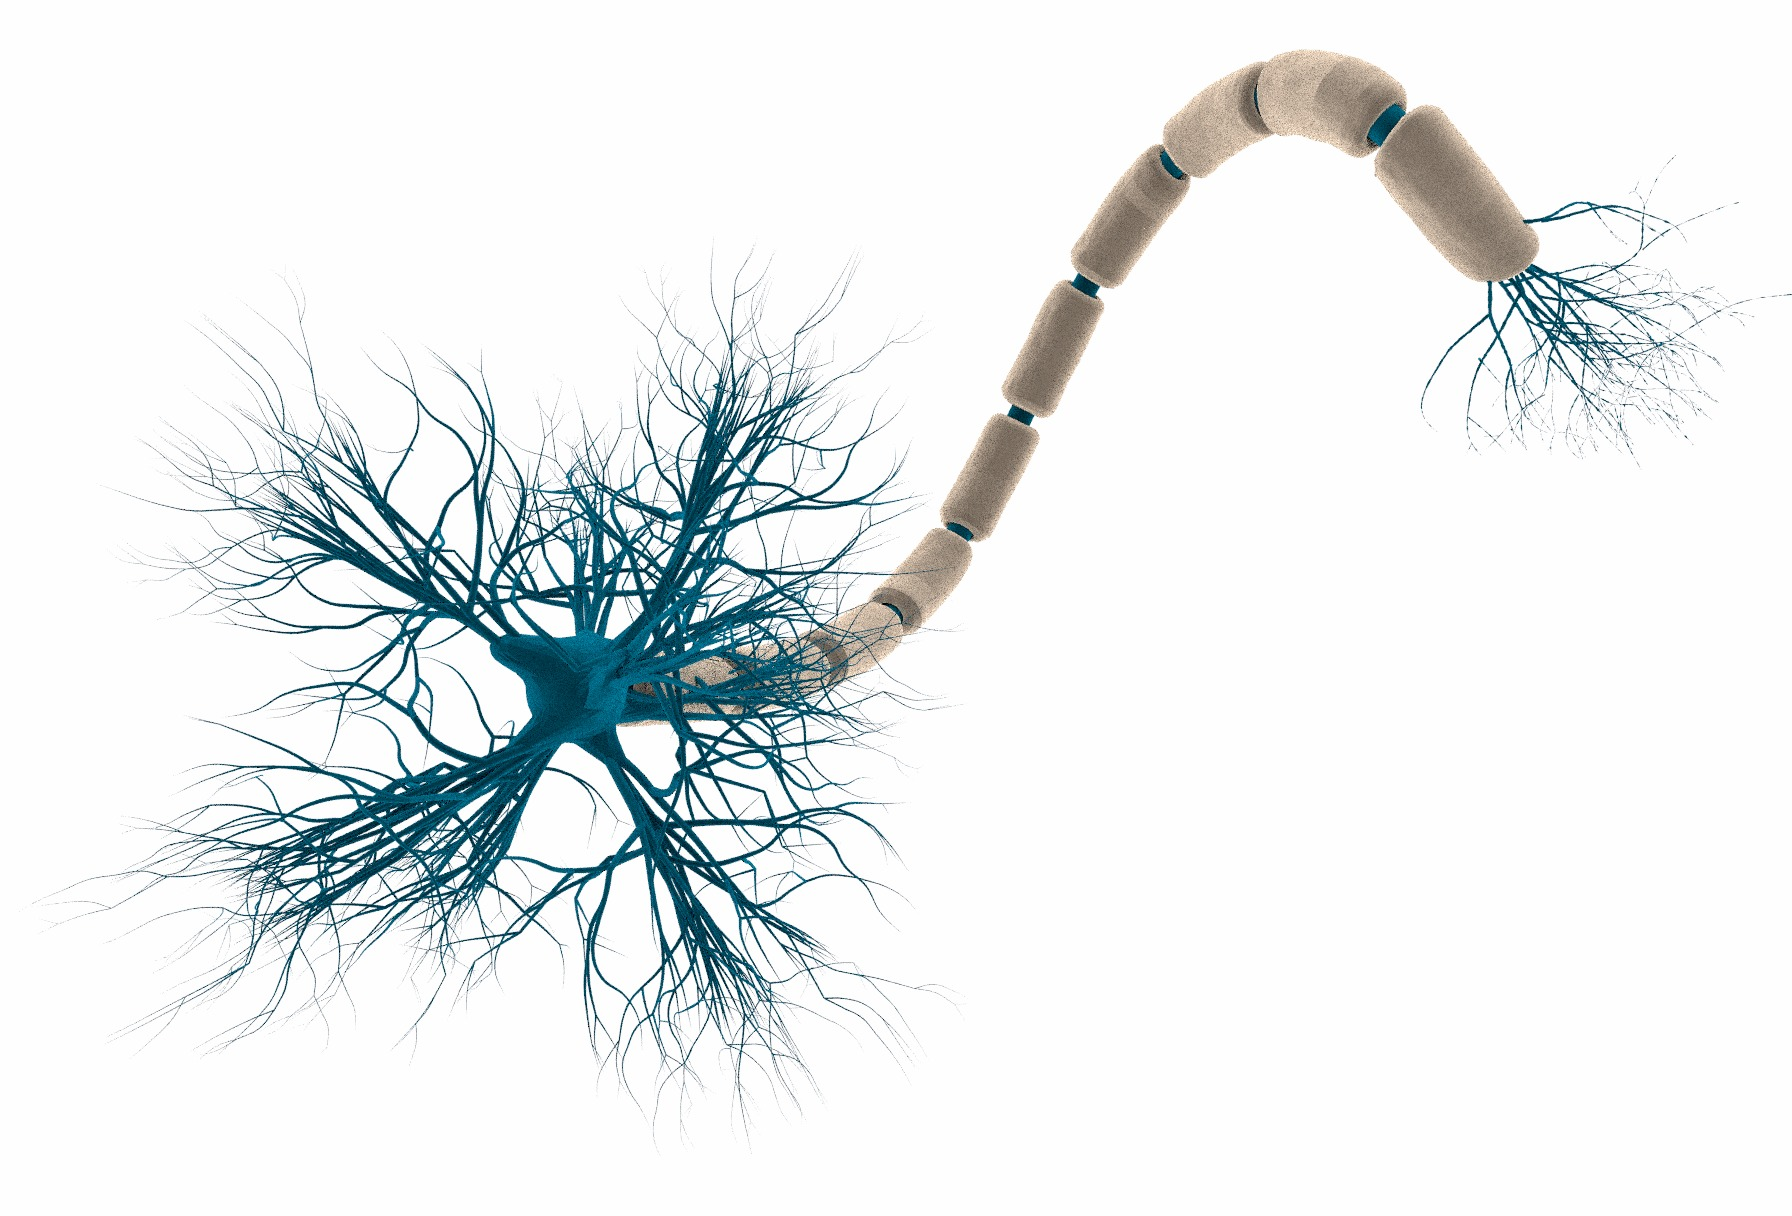
\includegraphics[width=0.8\textwidth]{neuron.jpg}  \end{figure}} 
\titlepage
\end{frame}

%%%%%%%%%%%%%%%%%%%%%%%%%%%%%%%%%%%%%%%%%%%%%%%%%%%%%%
%%%%%%%%%%%%%%%%%%%%%%%%%%%%%%%%%%%%%%%%%%%%%%%%%%%%%%
\begin{frame}{Wstęp}
\tableofcontents
\end{frame}

%%%%%%%%%%%%%%%%%%%%%%%%%%%%%%%%%%%%%%%%%%%%%%%%%%%%%%
%%%%%%%%%%%%%%%%%%%%%%%%%%%%%%%%%%%%%%%%%%%%%%%%%%%%%%
\section{\scshape Opis problemu}
\subsection{Model czworonoga}
\begin{frame}{Model czworonoga}

\begin{figure} 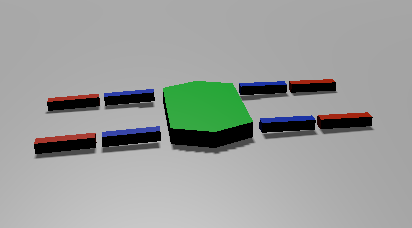
\includegraphics[width=\textwidth]{quadruped.png}  \end{figure}

\end{frame}

%%%%%%%%%%%%%%%%%%%%%%%%%%%%%%%%%%%%%%%%%%%%%%%%%%%%%%
%%%%%%%%%%%%%%%%%%%%%%%%%%%%%%%%%%%%%%%%%%%%%%%%%%%%%%
\section{\scshape Metodyka}
\subsection{Struktura sieci neuronowej}
\begin{frame}{Architektura sieci}
{
\begin{frame}
        \begin{tikzpicture}[remember picture,overlay]
            \node[at=(current page.center)] {
                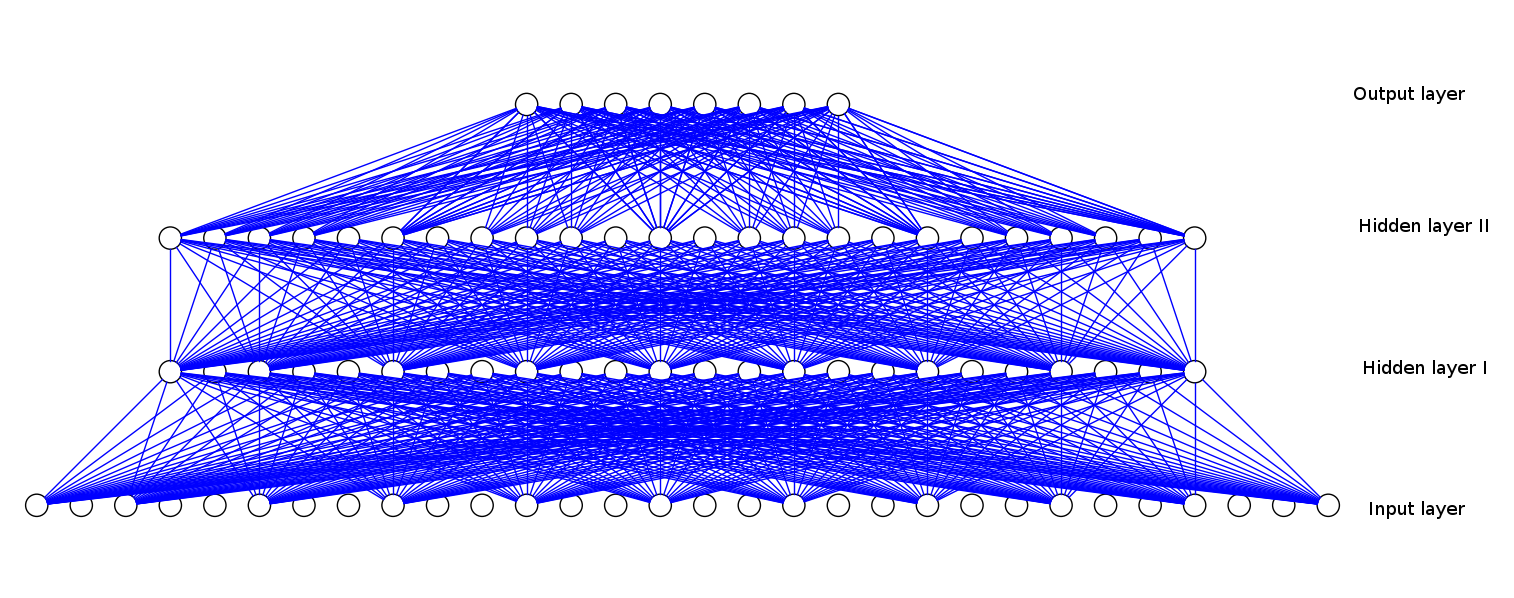
\includegraphics[width=\paperwidth]{net_cropped_caption.png}
            };
        \end{tikzpicture}
     \end{frame}
}
%\begin{figure} 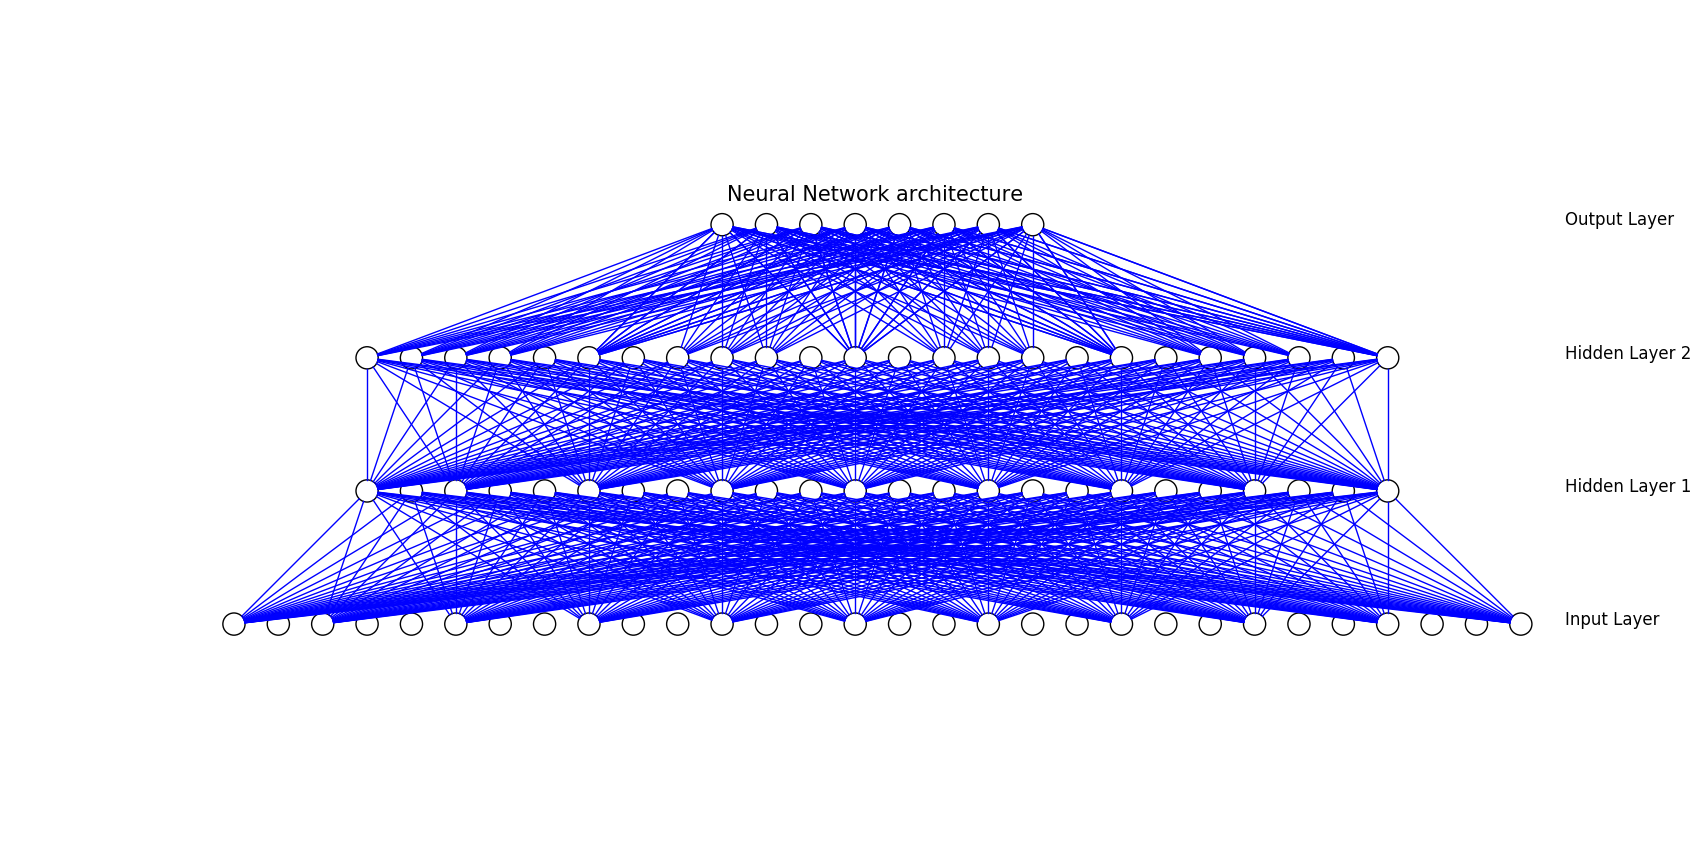
\includegraphics[width=\textwidth]{network_structure.png}  \end{figure}

\end{frame}
\subsection{Wejścia sieci}
\begin{frame}{Wejścia sieci}

\begin{itemize}
\item złe kroki
\item lokalna pozycja odnóży
\item lokalna pozycja tłuowia
\item liniowa prędkość ciała
\item prędkość kątowa ciała
\item dodatkowe cechy

%\item wrong movements for legs
%\item local orientation of legs
%\item local orientation of body 
%\item linear velocity of body
%\item angular velocity
%\item additional features
\end{itemize}

\end{frame}



%bge.logic.body[i].localOrientation.to_euler().x / pi
%bge.logic.body[i].localOrientation.to_euler().y / pi
%bge.logic.body[i].localOrientation.to_euler().z / pi
%bge.logic.body[i].localLinearVelocity.x / 3
%bge.logic.body[i].localLinearVelocity.y / 3
%bge.logic.body[i].localLinearVelocity.z / 3
%
%(bge.logic.legFL1[i].localOrientation * bge.logic.body[i].localOrientation.inverted()).to_euler().x / pi
%(bge.logic.legFL2[i].localOrientation * bge.logic.legFL1[i].localOrientation.inverted()).to_euler().x / pi
%
%(bge.logic.legFR1[i].localOrientation * bge.logic.body[i].localOrientation.inverted()).to_euler().x / pi
%(bge.logic.legFR2[i].localOrientation * bge.logic.legFR1[i].localOrientation.inverted()).to_euler().x / pi
%
%(bge.logic.legRL1[i].localOrientation * bge.logic.body[i].localOrientation.inverted()).to_euler().x / pi
%(bge.logic.legRL2[i].localOrientation * bge.logic.legRL1[i].localOrientation.inverted()).to_euler().x / pi
%
%(bge.logic.legRR1[i].localOrientation * bge.logic.body[i].localOrientation.inverted()).to_euler().x / pi
%(bge.logic.legRR2[i].localOrientation * bge.logic.legRR1[i].localOrientation.inverted()).to_euler().x / pi
%
%badhits = input[0][i][14] = (bge.logic.body[i]['hit'] + bge.logic.legFL1[i]['hit'] + bge.logic.legFR1[i]['hit'] + bge.logic.legRL1[i]['hit'] + bge.logic.legRR1[i]['hit']) / 5
%bge.logic.legFL2[i]['hit']
%bge.logic.legFR2[i]['hit']
%bge.logic.legRL2[i]['hit']
%bge.logic.legRR2[i]['hit']
%
%(bge.logic.legFL1[i].localAngularVelocity.x - bge.logic.body[i].localAngularVelocity.x) / 5
%(bge.logic.legFL2[i].localAngularVelocity.x - bge.logic.legFL1[i].localAngularVelocity.x) / 5
%
%(bge.logic.legFR1[i].localAngularVelocity.x - bge.logic.body[i].localAngularVelocity.x) / 5
%(bge.logic.legFR2[i].localAngularVelocity.x - bge.logic.legFR1[i].localAngularVelocity.x) / 5
%
%(bge.logic.legRL1[i].localAngularVelocity.x - bge.logic.body[i].localAngularVelocity.x) / 5
%(bge.logic.legRL2[i].localAngularVelocity.x - bge.logic.legRL1[i].localAngularVelocity.x) / 5
%
%(bge.logic.legRR1[i].localAngularVelocity.x - bge.logic.body[i].localAngularVelocity.x) / 5
%(bge.logic.legRR2[i].localAngularVelocity.x - bge.logic.legRR1[i].localAngularVelocity.x) / 5
%
%bge.logic.body[i].localAngularVelocity.x / 5
%bge.logic.body[i].localAngularVelocity.y / 5
%bge.logic.body[i].localAngularVelocity.z / 5
%

\subsection{Wyjścia sieci}
\begin{frame}{Wyjścia sieci}
\end{frame}
\subsection{Algorytm genetyczny}
\begin{frame}{Algorytm genetyczny}

	\begin{figure} 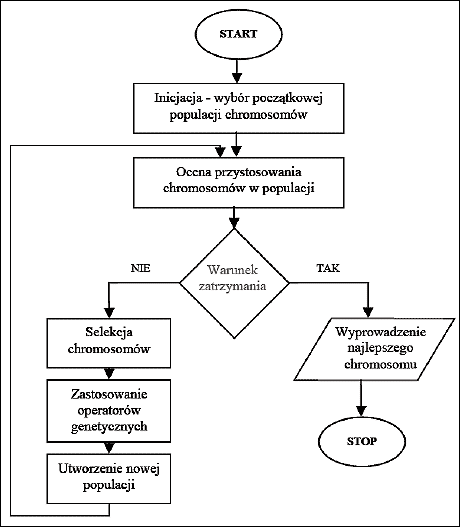
\includegraphics[width=0.6\textwidth]{schemat_ga.png}  \end{figure}

\end{frame}

\subsection{Narzędzia}
\begin{frame}{Narzędzia}
	\begin{itemize}
		\item{Blender 2.68} %\begin{figure} 
\includegraphics[width=0.4\textwidth]{blender.png}  \end{figure}}
		\item{Python 3.3.0} %\begin{figure} 
\includegraphics[width=0.4\textwidth]{python.png}  \end{figure}}

		\item{biblioteki: pybrain, numpy, plotly, scipy
                    \begin{figure}[!htb]
                    \minipage{0.25\textwidth}
                      
\includegraphics[width=\linewidth]{blender.png}
                    \endminipage\hfill
                    \minipage{0.14\textwidth}%
                      
\includegraphics[width=\linewidth]{plotly.jpg}
                    \endminipage

                    \minipage{0.25\textwidth}
                      
\includegraphics[width=\linewidth]{python.png}
                    \endminipage\hfill
%                    \end{figure}			
%                    \begin{figure}[!htb]

                    \minipage{0.25\textwidth}
                      
\includegraphics[width=\linewidth]{pybrain.png}
                    \endminipage\hfill
                    \minipage{0.14\textwidth}%
                      \includegraphics[width=\linewidth]{scipy.png}
                    \endminipage

                    \minipage{0.25\textwidth}
                      
\includegraphics[width=\linewidth]{numpy.jpg}
                    \endminipage\hfill

                    \end{figure}			
			}
	\end{itemize}
\end{frame}


%%%%%%%%%%%%%%%%%%%%%%%%%%%%%%%%%%%%%%%%%%%%%%%%%%%%%%
%%%%%%%%%%%%%%%%%%%%%%%%%%%%%%%%%%%%%%%%%%%%%%%%%%%%%%
\subsection{Funkcja przystosowania}
\begin{frame}{Funkcja przystosowania}

	\begin{figure} 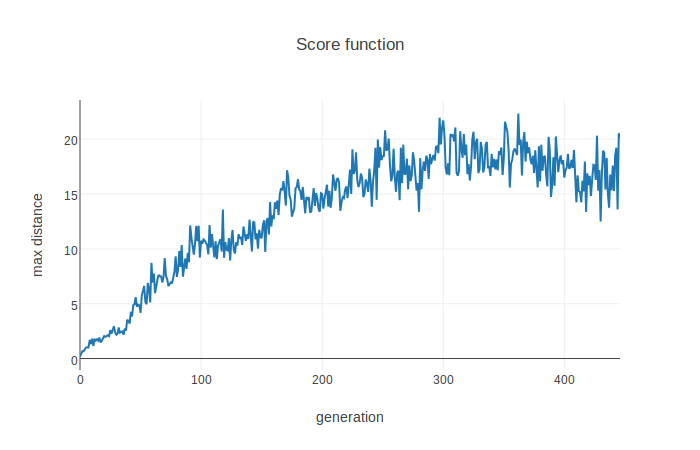
\includegraphics[width=\textwidth]{score_function.png}  \end{figure}


\end{frame}

%%%%%%%%%%%%%%%%%%%%%%%%%%%%%%%%%%%%%%%%%%%%%%%%%%%%%%
%%%%%%%%%%%%%%%%%%%%%%%%%%%%%%%%%%%%%%%%%%%%%%%%%%%%%%
\section{\scshape Wyniki}
\subsection{Nauka chodzenia}
\begin{frame}{Nauka chodzenia}
\begin{center}
\movie[
  height = 6cm,
  width = 10cm,
  showcontrols,
  poster
] 
{}{videonnga.mp4}	
\end{center}
\end{frame}

\end{document}
